\chapter{Results and discussion}

\section{Characteristics of q\textsubscript{1} - q\textsubscript{2} stability diagrams for one electron}

%\subsection{Comparison of simulation and determinant stability criterion}

We will start by looking at the stability diagrams for different $\nicefrac{\Omega_2}{\Omega_1}$ ratios. Starting with \ref{fig:stabil-eta=3}.

\begin{figure}[H]
\begin{subfigure}{.5\textwidth}
  \centering
  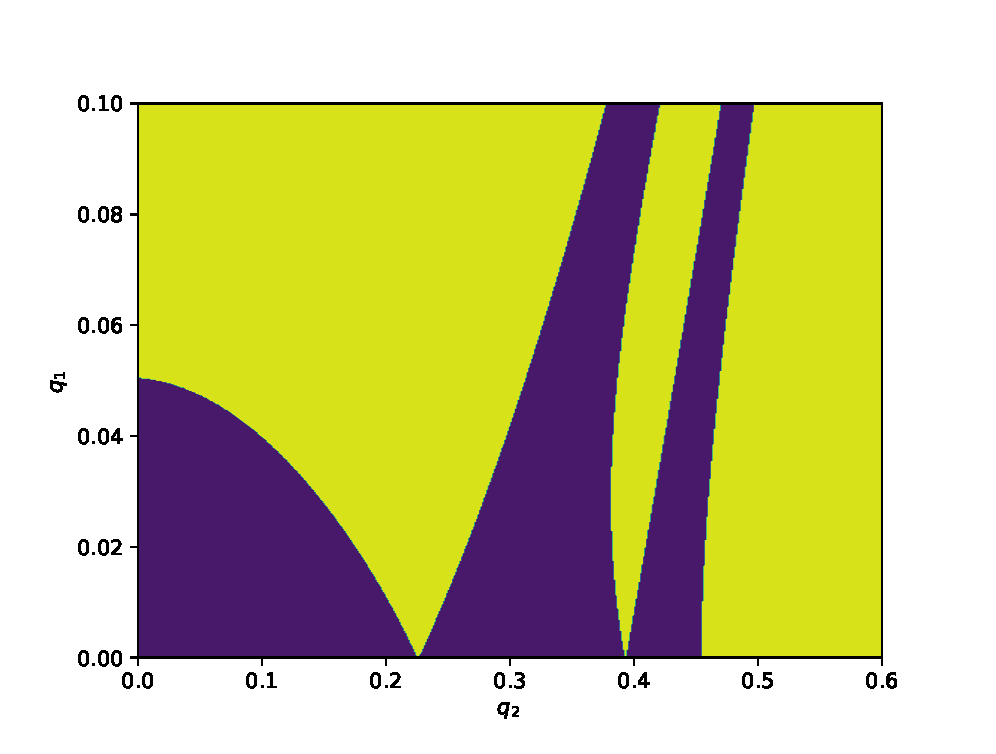
\includegraphics[width=\linewidth]{img/q1_0.0-0.1_q2_0.0-0.6_500x500_3.eps}
  \caption{Determinant}
  \label{fig:det_3}
\end{subfigure}%
\begin{subfigure}{.5\textwidth}
  \centering
  \includegraphics[width=\linewidth]{img/0_ions_1_electrons_q1_0.0-0.1_q2_0.0-0.55_960x960_3_400.eps}  
  \caption{Simulation}
  \label{fig:sim_3}
\end{subfigure}
\caption{Stability diagrams for $\nicefrac{\Omega_2}{\Omega_1} = 3$}
\label{fig:stabil-eta=3}
\end{figure}

In the sub-figure \ref{fig:det_3} we can see stable\textit{(dark)} and unstable\textit{(light)} regions of the studied differential equation. The image \ref{fig:sim_3} combines two pictures. The red curve indicates the edge of stability regions $\rightarrow$ the region under the curve is stable. In the background is a contour plot of the average electron velocity throughout the trajectory relative to the initial velocity. The color bar to the right indicates the value of this ratio.

Moving to larger frequency ratio $\rightarrow \nicefrac{\Omega_2}{\Omega_1} = 13$ we can start to notice some patterns.

\begin{figure}[H]
\begin{subfigure}{.5\textwidth}
  \centering
  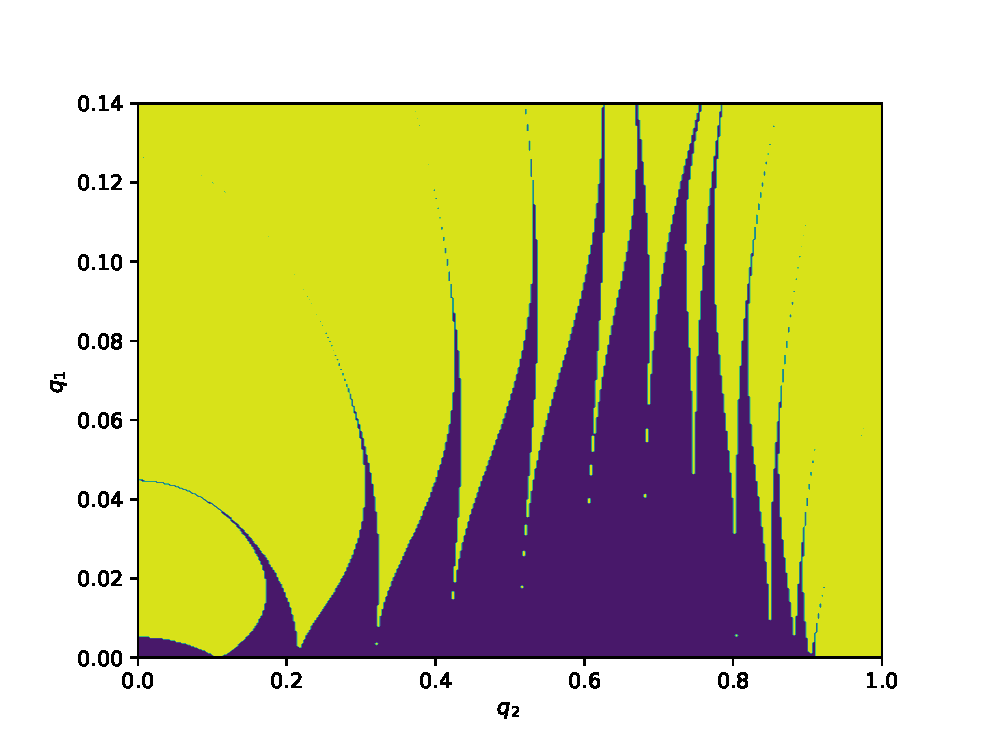
\includegraphics[width=\linewidth]{img/q1_0.0-0.14_q2_0.0-1.0_400x400_13.eps}
  \caption{Determinant}
  \label{fig:det_13}
\end{subfigure}%
\begin{subfigure}{.5\textwidth}
  \centering
  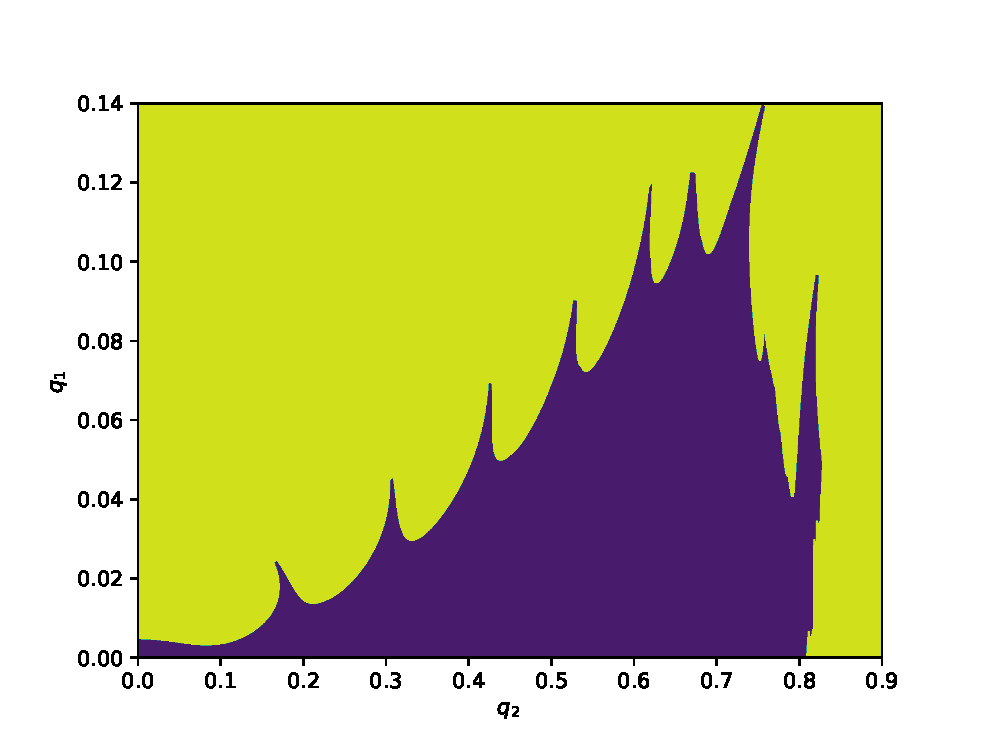
\includegraphics[width=\linewidth]{img/0_ions_1_electrons_q1_0.0-0.14_q2_0.0-0.9_1296x1296_13.eps}  
  \caption{Simulation}
  \label{fig:sim_13}
\end{subfigure}
\caption{Stability diagrams for $\nicefrac{\Omega_2}{\Omega_1} = 13$}
\label{fig:stabil-eta=3}
\end{figure}


\subsection{Dependence on initial conditions}

\section{Creating a Coulomb crystal}

\section{Stability of electron in Coulomb crystal}
\subsection{One electron - one ion}
\subsection{One electron - twenty ions}
\subsection{One electron - a hundred ions}